\section{Теоритические сведения}
\begin{figure}[ht!]
    \center{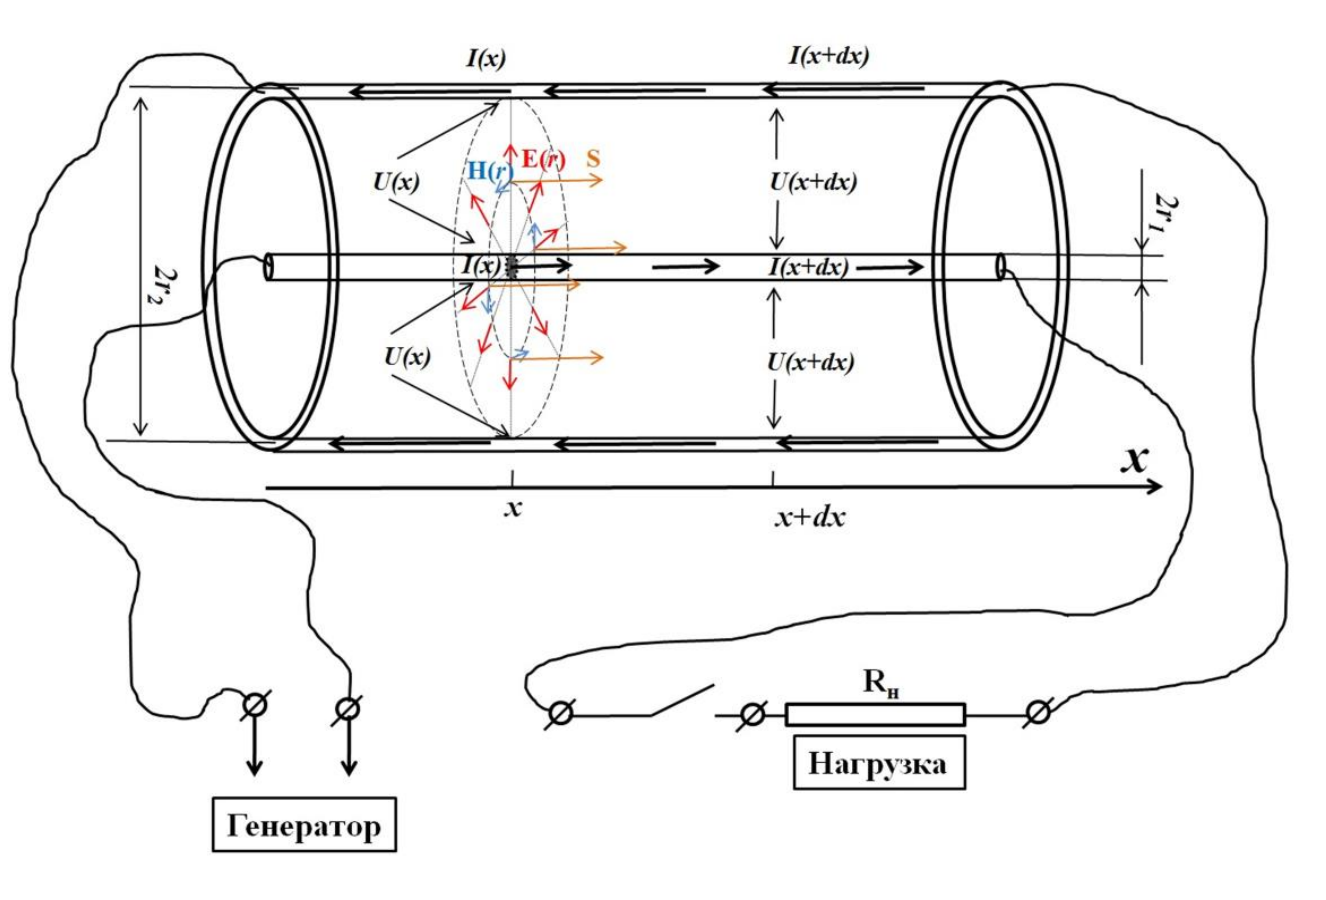
\includegraphics[width=0.8\linewidth]{../img/fig1.png}}
\end{figure}


Рассмотрим элемент $dx$ длинного коаксиального кабеля. Этот элемент представляет
собой изолированный коаксиальный проводящий (медный) цилиндр некоторого радиуса
$r_{2}$, на оси которого расположен сплошной тонкий проводник (медный) круглого сечения с
радиусом $r_{1}$.  Пространство между этими проводниками заполнена средой, обладающей
диэлектрической проницаемостью $ \varepsilon$ и магнитной восприимчивостью $ \mu$.
 Как известно, такой элемент обладает индуктивностью
 \[
     dL = 2 \mu\ln\left(r_{2}/r_{1}\right)dx
 \]
 Удельная (погонная) индуктивность единицы длины такого кабеля:
 \[
     L_{x} = \frac{dL}{dx} = 2\mu\ln\left(r_{2}/r_{1}\right)
 \]
 Два проводника, образующих этот элемент $dx$  коаксиального кабеля, должны обладать
 взаимной ёмкостью. Можно показать, что ёмкость элемента $dx$  коаксиального кабеля
 определяется выражением:
 \[
     dC = \frac{ \varepsilon}{2\ln\left(r_{2}/r_{1}\right)}dx
 \]
 а его удельная (погонная) ёмкость единицы длины равна:
 \[
     C_{x} = \frac{dC}{dx} = \frac{ \varepsilon}{2\ln\left(r_{2}/r_{1}\right)}
 \]
 
 Когда по такому кабелю передаётся сигнал, в его центральной жиле и внешней оболочке
 возникают взаимно противоположные токи $I(x)$,  а также электрическое напряжение $U(x)$
 между внешним и внутренним проводниками. При высоких частотах $\nu$ сигналов,
 распространяющихся в кабеле (когда длина кабеля $l\gg V/\nu$, где $V$~--- характерная скорость
 распространения сигнала в кабеле,  эта скорость, как правило, порядка скорости света)
 $I(x)$ и $U(x)$ вообще говоря зависят от координаты $x$.

 Изменение напряжения на концах элемента $dx$ вызваны возникновением ЭДС индукции и
 падением напряжения в результате омического сопротивления проводников:
 \[
     U(x+dx) - U(x) = -\frac{L_{x}dx}{c^{2}}\frac{\partial I}{\partial t} - R_{x}dxI,
 \]
где  погонное сопротивление
\[
    R_{x} = \frac{dR}{dx} = \frac{1}{ \sigma S}
\]
$ \sigma$~--- удельная проводимость материала проводников, $S$~--- площадь их поперечного сечения.

Изменение силы тока вызвано тем, что некоторая часть электрического заряда $q$ как бы
<<перетекает на <<обкладки>>  конденсатора, роль которых играют проводники коаксиального кабеля:
\[
    I(x+dx) - I(x) = -\frac{\partial q}{\partial t }
\]
где $q=C_{x} dx U$.

Итого
\begin{equation}
    \begin{cases}
        U(x) = U(x+dx) + \frac{L_{x}dx}{c^{2}}\frac{\partial I}{\partial t} + R_{x}dxI\\
        I(x) = I(x+dx) + \frac{\partial q}{\partial t}  
    \end{cases}
\end{equation}

Эту систему уравнений называют телеграфными уравнениями. Разделим оба уравнения на $dx$
и перепишем уравнения:
\begin{equation}
\begin{cases}
    \frac{\partial I}{\partial x} = -C_{x} \frac{\partial U}{\partial t} \\
    \frac{\partial U}{\partial x} = -\frac{L_{x}}{c^{2}}\frac{\partial I}{\partial t} - R_{x}I 
\end{cases}
\end{equation}

Получаем волновое уравнение для напряжения
\[
    \frac{\partial^{2}U}{\partial t^{2}} - V_{\text{ф}}\frac{\partial^{2}U}{\partial x^{2}} + \gamma \frac{\partial U}{\partial t} = 0
\]
где
\[
    V_{\text{ф}} = \frac{c}{\sqrt{L_{x}C_{x}}}
\]
\[
    \gamma = R_{x}C_{x}V_{\text{ф}}^{2}
\]

\[
    V_{\text{ф}} = \frac{c}{\sqrt{ \varepsilon \mu}}
\]

Решение удобно искать в виде
\[
    U(x, t) = U_{0} e^{-iwt}e^{\left(- \alpha + ik\right)x}
\]
\[
    I(x, t) = U_{0} \frac{C_{x}w}{k+i \alpha}e^{-iwt}e^{\left(- \alpha + ik\right)x}
\]
Волновое сопротивление
\[
    Z(w, k) = \frac{U(x, t)}{I(x, t)} = \frac{k+i \alpha}{C_{x}w}
\]
не зависит от времени и координаты.

В пределах малых затуханий $ \alpha\ll w$ 
\[
    Z(w, k) \approx \frac{k}{C_{x}w}= \frac{1}{C_{x}V_{\text{ф}}} = \frac{1}{c}\sqrt{\frac{L_{x}}{C_{x}}}
\]
Если в конце такую длинную линию замкнуть на сопротивление
\[
    R_{0} = \frac{1}{c}\sqrt{\frac{L_{x}}{C_{x}}}
\]
то бегущая вдоль длинной линии волна <<будет воспринимать>> нагрузку как бесконечное
продолжение этой длинной линии. Другими словами, когда длинная линия подключена к
нагрузке с сопротивлением $R_{0}$, отражённой волны не возникает. Во всех остальных
случаях, когда $R \neq R_{0}$  (в том числе и в частных случаях незамкнутого конца, когда
$R \to \infty$  и короткозамкнутой линии, когда $R=0$)  возникает отражённая волна,
описываемая выражением
\[
    U(x, t) = U_{0}e^{-iwt}e^{-\left( \alpha + ik\right)x}
\]

Характеристическое уравнение
\[
    -w^{2} - V_{\text{ф}}^{2}\left(- \alpha + ik\right)^{2} - iw \gamma = 0
\]

Отсюда следует
\[
    \alpha\approx R_{x}C_{x}\frac{V_{\text{ф}}}{2}
\]
\[
    k=\frac{w}{V_{\text{ф}}}
\]

Таким образом, амплитуда напряжения на нагрузке (в конце длинной линии) будет иметь вид
\[
    U_{\text{н}}(t) = U_{0}e^{- \alpha l + ikl - iwt}
\]
При этом амплитуда и набег фазы имеют вид
\[
    U_{\text{н}} = U_{0}e^{- \alpha l}
\]
\[
    \Delta \varphi = kl
\]
Так как модуль волнового вектора $k$ прямо пропорционален частоте сигнала $w$, то
$ \Delta \varphi$    монотонно увеличивается с увеличением $w$.

Декремент затухания и волновое число легко определить из эксперимента
\[
    \alpha(w) = \frac{1}{l}\ln\left(\frac{U_{0}}{U_{\text{н}}}\right)   
\]
\[
    k=\frac{ \Delta \varphi}{l}
\]

